\documentclass{ctexart}
\usepackage{graphicx}
\usepackage{float}
\usepackage{amsmath}
\usepackage{amsfonts}
\usepackage{amssymb}
\usepackage{tikz}
\usetikzlibrary{shapes.geometric, arrows}
\tikzstyle{startstop} = [rectangle, rounded corners, minimum width=3cm, minimum height=1cm,text centered, draw=black, fill=red!30]
\tikzstyle{io} = [trapezium, trapezium left angle=70, trapezium right angle=110, minimum width=3cm, minimum height=1cm, text centered, draw=black, fill=blue!30]
\tikzstyle{process} = [rectangle, minimum width=3cm, minimum height=1cm, text centered, draw=black, fill=orange!30]
\tikzstyle{decision} = [diamond, minimum width=3cm, minimum height=1cm, text centered, draw=black, fill=green!30]
\tikzstyle{arrow} = [thick,->,>=stealth]
\usepackage[a4paper, top=3cm, bottom=3cm, left=3cm, right=3cm]{geometry}
\usepackage{subcaption}
\usepackage{xcolor}
\usepackage{listings}
\lstset{
	keywordstyle=\color{blue!70},
	commentstyle=\color{red!50!green!50!blue!50},
	frame=shadowbox,
	rulesepcolor=\color{red!20!green!20!blue!20},
	tabsize=2,
	basicstyle=\ttfamily\small,
	numberstyle=\tiny,
	numbers=left,
	showstringspaces=false,
	breaklines=true,
	language=MATLAB
}
\title{遥感综合实验实验报告\\遥感图像预处理}
\author{蓝彧文~16020710017}
\begin{document}
	\maketitle
	\tableofcontents
	\newpage
	\section{实验一~图像滤波}
	\subsection{实验目的}
设计和使用低通滤波器,滤除分布在图像中的高斯白噪声。
\subsection{实验原理}
\subsubsection{高斯白噪声}
高斯白噪声是一种理想的噪声模型。高斯白噪声中,噪声振幅值是服从正态分布的。
\[ f(x)=\frac{1}{\sqrt{2\pi}\sigma}\mathrm{e}^{-\frac{(x-\mu)^2}{2\sigma^2}} \]
它的振幅分布直方图如下图\ref{fig:gwnhistogram}所示。
\begin{figure}[H]
	\centering
	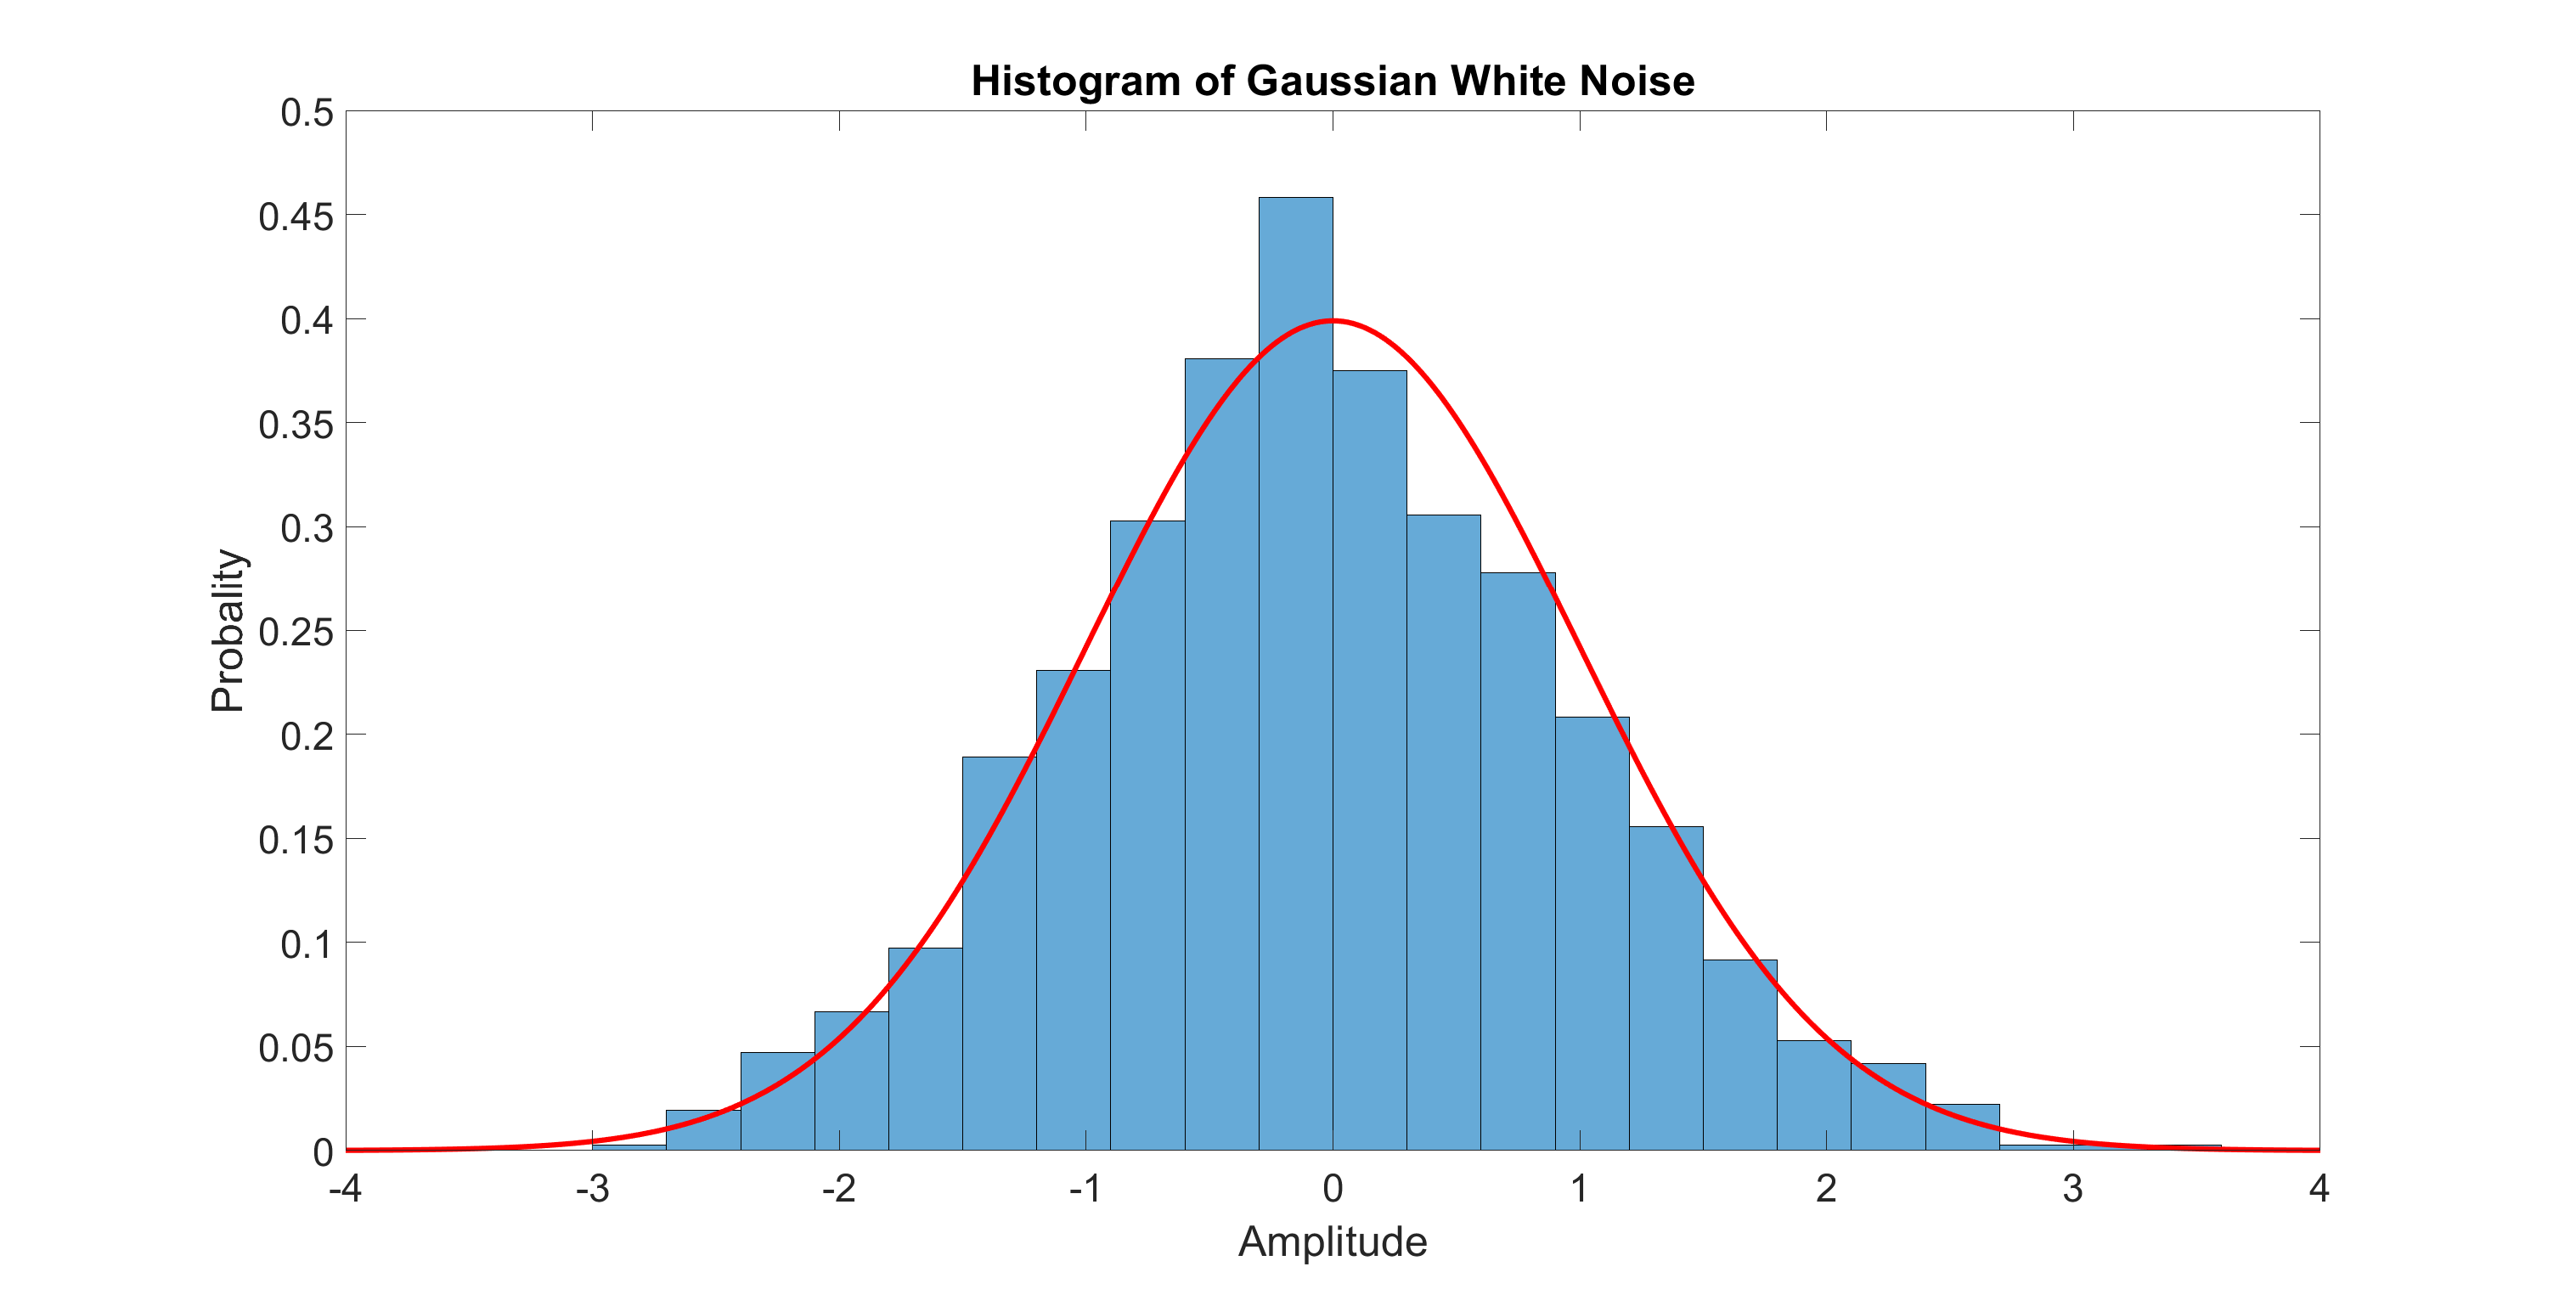
\includegraphics[width=0.7\linewidth]{figure/gwn_histogram}
	\caption{高斯白噪声幅度概率分布}
	\label{fig:gwnhistogram}
\end{figure}
它的功率谱是在频域内均匀分布的,在无限宽频带内满足
\[ G(\omega) = \frac{N_0}{2},\quad -\infty<\omega<+\infty \]
它的自相关函数为为
\[ R(\tau) = \frac{1}{2\pi}\int_{-\infty}^{+\infty}G(\omega)\mathrm{e}^{\mathrm{j}\omega t}\mathrm{d}\omega=\frac{N_0}{2}\delta(\tau) \]

在数字图像中,高斯白噪声线性叠加在图像中。设$f(x, y)$为原图像的表达式,$v(x, y)$为噪声在时空域上的表达式,则包含噪声的图像表达为
\[ g(x, y) = f(x, y) + v(x, y)\]
\subsubsection{傅里叶变换}
傅里叶变换是一种常用的信号分析方法。对于在时空上分布的二数字维图像$f(x, y)$,有傅里叶变换
\[ F(u, v) = \sum_{n = 0}^{N - 1}\sum_{m = 0}^{M - 1}\mathrm{e}^{-\mathrm{j}(\omega_kn+\omega_lm)}f(n, m) \]
\subsubsection{低通滤波器}
\subsection{实验流程}
\subsection{实验程序}
\subsection{实验结果和分析}
	\section{实验二~图像变换}
	\subsection{实验目的}
学习和实践图像翻转、对数变换、幂次变换等图像处理方法。学习使用算术、逻辑操作实现图像增强。
\subsection{实验原理}
\subsubsection{图像反转}
对于二维灰度图像可以执行计算
\[ s=L-1-r \]
重新计算每一个像素点的像素值。这样计算之后得到的图像即为反转后的图像。图像反转会使得原本在图像中是明亮的区域变成黑暗的区域、黑暗的区域变成明亮的区域。
\subsubsection{对数变换}
对于二维灰度图像可以执行计算
\[ s=c\log(1+r) \]
重新计算每一点的像素值。这样的计算,可以提高图像在暗部或明部细节的辨识度。%例如,一个图像的能量主要集中在比较暗的部分,即在图像中暗部保存了许多细节,正常显示的时候会显得图像细节难以辨认。如果对这样的图像进行对数变换,那么就使得暗部的像素点的值得到提升,提高了图像在暗部的可辨识性。
\subsubsection{幂次变换}
对于二维的灰度图像可以执行计算
\[ s=cr^b \]
重新计算每一点的像素值。$c$和$b$为正常数,当$b$取不同值时将得到不同的变换曲线。
\subsubsection{使用算术、逻辑操作进行增强}
对两幅或多幅图像进行计算,进行求比值、求差值计算。可以实现从不同时期的遥感数据中分析出地表特征的变化。
\subsection{实验流程}
\begin{tikzpicture}[node distance=1.5cm]
\node(start) [startstop] {开始};
\node(input_img) [io, text width=2cm] {读取二维灰度图片};
\node(power) [process] {进行幂次变换};
\node(log) [process] {进行对数变换};
\node(plot) [process] {绘制变换曲线};
\node(output_img) [io, text width=2cm] {输出变换后的图片};
\node(output_graph) [io, text width=2cm] {输出绘制的变换曲线};
\node(input_rsimg) [io, text width=2cm] {读取具有差异的两幅遥感图像};
\node(process_rsimg) [process] {选择合适的变换对遥感图像进行处理};
\node(output_rsimg) [io, text width=2cm] {输出处理后的遥感图像};
\node(end) [startstop] {结束};

\draw[arrow] (start) -- (input_img);
\draw[arrow] (input_img) -- (power);
\draw[arrow] (power) -- (log);
\draw[arrow] (log) -- ()
\end{tikzpicture}
\subsection{实验程序}
\subsection{实验结果和分析}
	\section{实验三~图像融合}
	\subsection{实验目的}
掌握一些基本的图像融合方法,包括基于像素灰度值的简单图像融合算法,以及彩色图像的分解于合成。完成遥感图像的图像融合。
\subsection{实验原理}
\subsubsection{图像融合的概念}
综合和提取两个或多个圆的图像信息,获得对同一场景或者目标更为准确、全面、可靠的图像,使之更适合人眼感知或计算机后续处理。
\begin{figure}[H]
	\centering
	\includegraphics[width=0.7\linewidth]{figure/fusion_flowchart.png}
	\caption{图像融合算法流程图}
	\label{fig:fusion_flowchart}
\end{figure}
\subsubsection{简单的图像融合算法}
\begin{description}
	\item[像素灰度值平均或加权平均法]
	\[ I(x, y)=\frac{\sum_{n=1}^{N}W^n(x, y)I^n(x, y)}{\sum_{n=1}^{N}W^n(x, y)} \]
	\[ W^n(x, y)=\frac{1}{N} \]
	\item[像素灰度值选大法] 
	\[ I(x, y)=\max_n\{I^n(x, y),\quad n=1,2,\dots N\} \]
	\item[像素灰度值选小法] 
	\[ I(x, y)=\min_n\{I^n(x, y),\quad 1,2,\dots N\} \]
\end{description}
\subsubsection{彩色图像的分解与合成}
\begin{description}
	\item[能量图像] 
	\[ I=Ir+Ig+Ib \]
	\item[变换后的彩色图像合成]
	蓝色分量:加高斯噪声污染
	
	绿色分量:进行对数变换
	
	红色分量:进行图像反转
	
	重新合成彩色图像
\end{description}
\subsubsection{彩色图像合成}
通过图像变换与融合突出图像中感兴趣的目标。
\subsubsection{通过图像融合得到变化检测差异图}
\begin{description}
	\item[差异图像] 
	\[ I1=1-\min \left( \frac{\mu_1}{\mu_2},\frac{\mu_2}{\mu_1} \right)  \]
	\[ I2= \left| \log\frac{X_2}{X_1} \right| = \left| \log X_2 - \log X_1 \right|  \]
	\item[图像融合]
	两个差异图的低频成分平均融合,高频成分取小融合。
\end{description}
\subsection{实验流程}
\begin{figure}[H]
	\centering
	\begin{tikzpicture}[node distance=1.5cm]
	\node(start) [startstop] {开始};
	\node(inputimg) [io, below of=start] {读取图片};
	\node(separateimg) [process, below of=inputimg] {分离彩色图像颜色通道};
	\node(fusionchannels) [process, below of=separateimg] {加权合并各通道能量};
	\node(outputenergyimg) [io, below of=fusionchannels] {输出能量合成图像};
	\node(channelcompare) [process, below of=outputenergyimg] {使用图片的两个不同通道进行对比};
	\node(outputchannelcomparation) [io, below of=channelcompare] {输出比较的结果};
	\node(channeltransform) [process, below of=outputchannelcomparation] {对各个通道分别进行变换};
	\node(outputtransformed) [io, below of=channeltransform] {输出变换后的图像};
	\node(inputmask) [io, below of=outputtransformed] {输入兴趣区域蒙版};
	\node(interestedarea) [process, below of=inputmask] {合成兴趣区域图像};
	\node(outputinterestedarea) [io, below of=interestedarea] {输出兴趣区域图像};
	\node(end) [startstop, below of=outputinterestedarea] {结束};
	
	\draw[arrow] (start) -- (inputimg);
	\draw[arrow] (inputimg) -- (separateimg);
	\draw[arrow] (separateimg) -- (fusionchannels);
	\draw[arrow] (fusionchannels) -- (outputenergyimg);
	\draw[arrow] (outputenergyimg) -- (channelcompare);
	\draw[arrow] (channelcompare) -- (outputchannelcomparation);
	\draw[arrow] (outputchannelcomparation) -- (channeltransform);
	\draw[arrow] (channeltransform) -- (outputtransformed);
	\draw[arrow] (outputtransformed) -- (inputmask);
	\draw[arrow] (inputmask) -- (interestedarea);
	\draw[arrow] (interestedarea) -- (outputinterestedarea);
	\draw[arrow] (outputinterestedarea) -- (end);
	\end{tikzpicture}
\end{figure}
\subsection{实验程序}
\lstinputlisting[caption={生成彩色图像的能量图像程序}]{"../Executable Script/Exp 3/ColorImageEnergyGraph.m"}
\lstinputlisting[caption={彩色图像的分解变换与合成程序}]{"../Executable Script/Exp 3/ColorImageTransformAndFusion.m"}
\lstinputlisting[caption={生成彩色图像的通道差异程序}]{"../Executable Script/Exp 3/ColorImageChannelsDiffer.m"}
\lstinputlisting[caption={$I_1=1-\min\left(\frac{\mu_1}{\mu_2},\frac{\mu_2}{\mu_1} \right) $差异图像生成函数}]{"../Function Library/ImageDiffer_Minus.m"}
\lstinputlisting[caption={$I_1=\left|\log X_1-\log X_2 \right| $差异图像生成函数}]{"../Function Library/ImageDiffer_Log.m"}
\lstinputlisting[caption={差异图像融合函数}]{"../Function Library/ImageDiffer.m"}
\lstinputlisting[caption={在图中标记兴趣区域程序}]{"../Executable Script/Exp 3/MarkInterestArea.m"}
\lstinputlisting[caption={图像加权融合函数}]{"../Function Library/SafetyConstantImageMultiply.m"}
\subsection{实验结果和分析}
\subsubsection{生成彩色图像的能量图像}
对原图片的红色、绿色和蓝色通道按照1、1、1的权重进行加权融合并重新进行量化,即可得到融合了红绿蓝三通道能量的能量图像,如图\ref{fig:dji0027energy}所示。
\begin{figure}[H]
	\centering	
	\begin{minipage}{0.45\linewidth}
		\includegraphics[width=\linewidth]{figure/DJI_0027_Compressed.png}
		\caption{原图片}
		\label{fig:dji0027original}
	\end{minipage}
	\begin{minipage}{0.45\linewidth}
		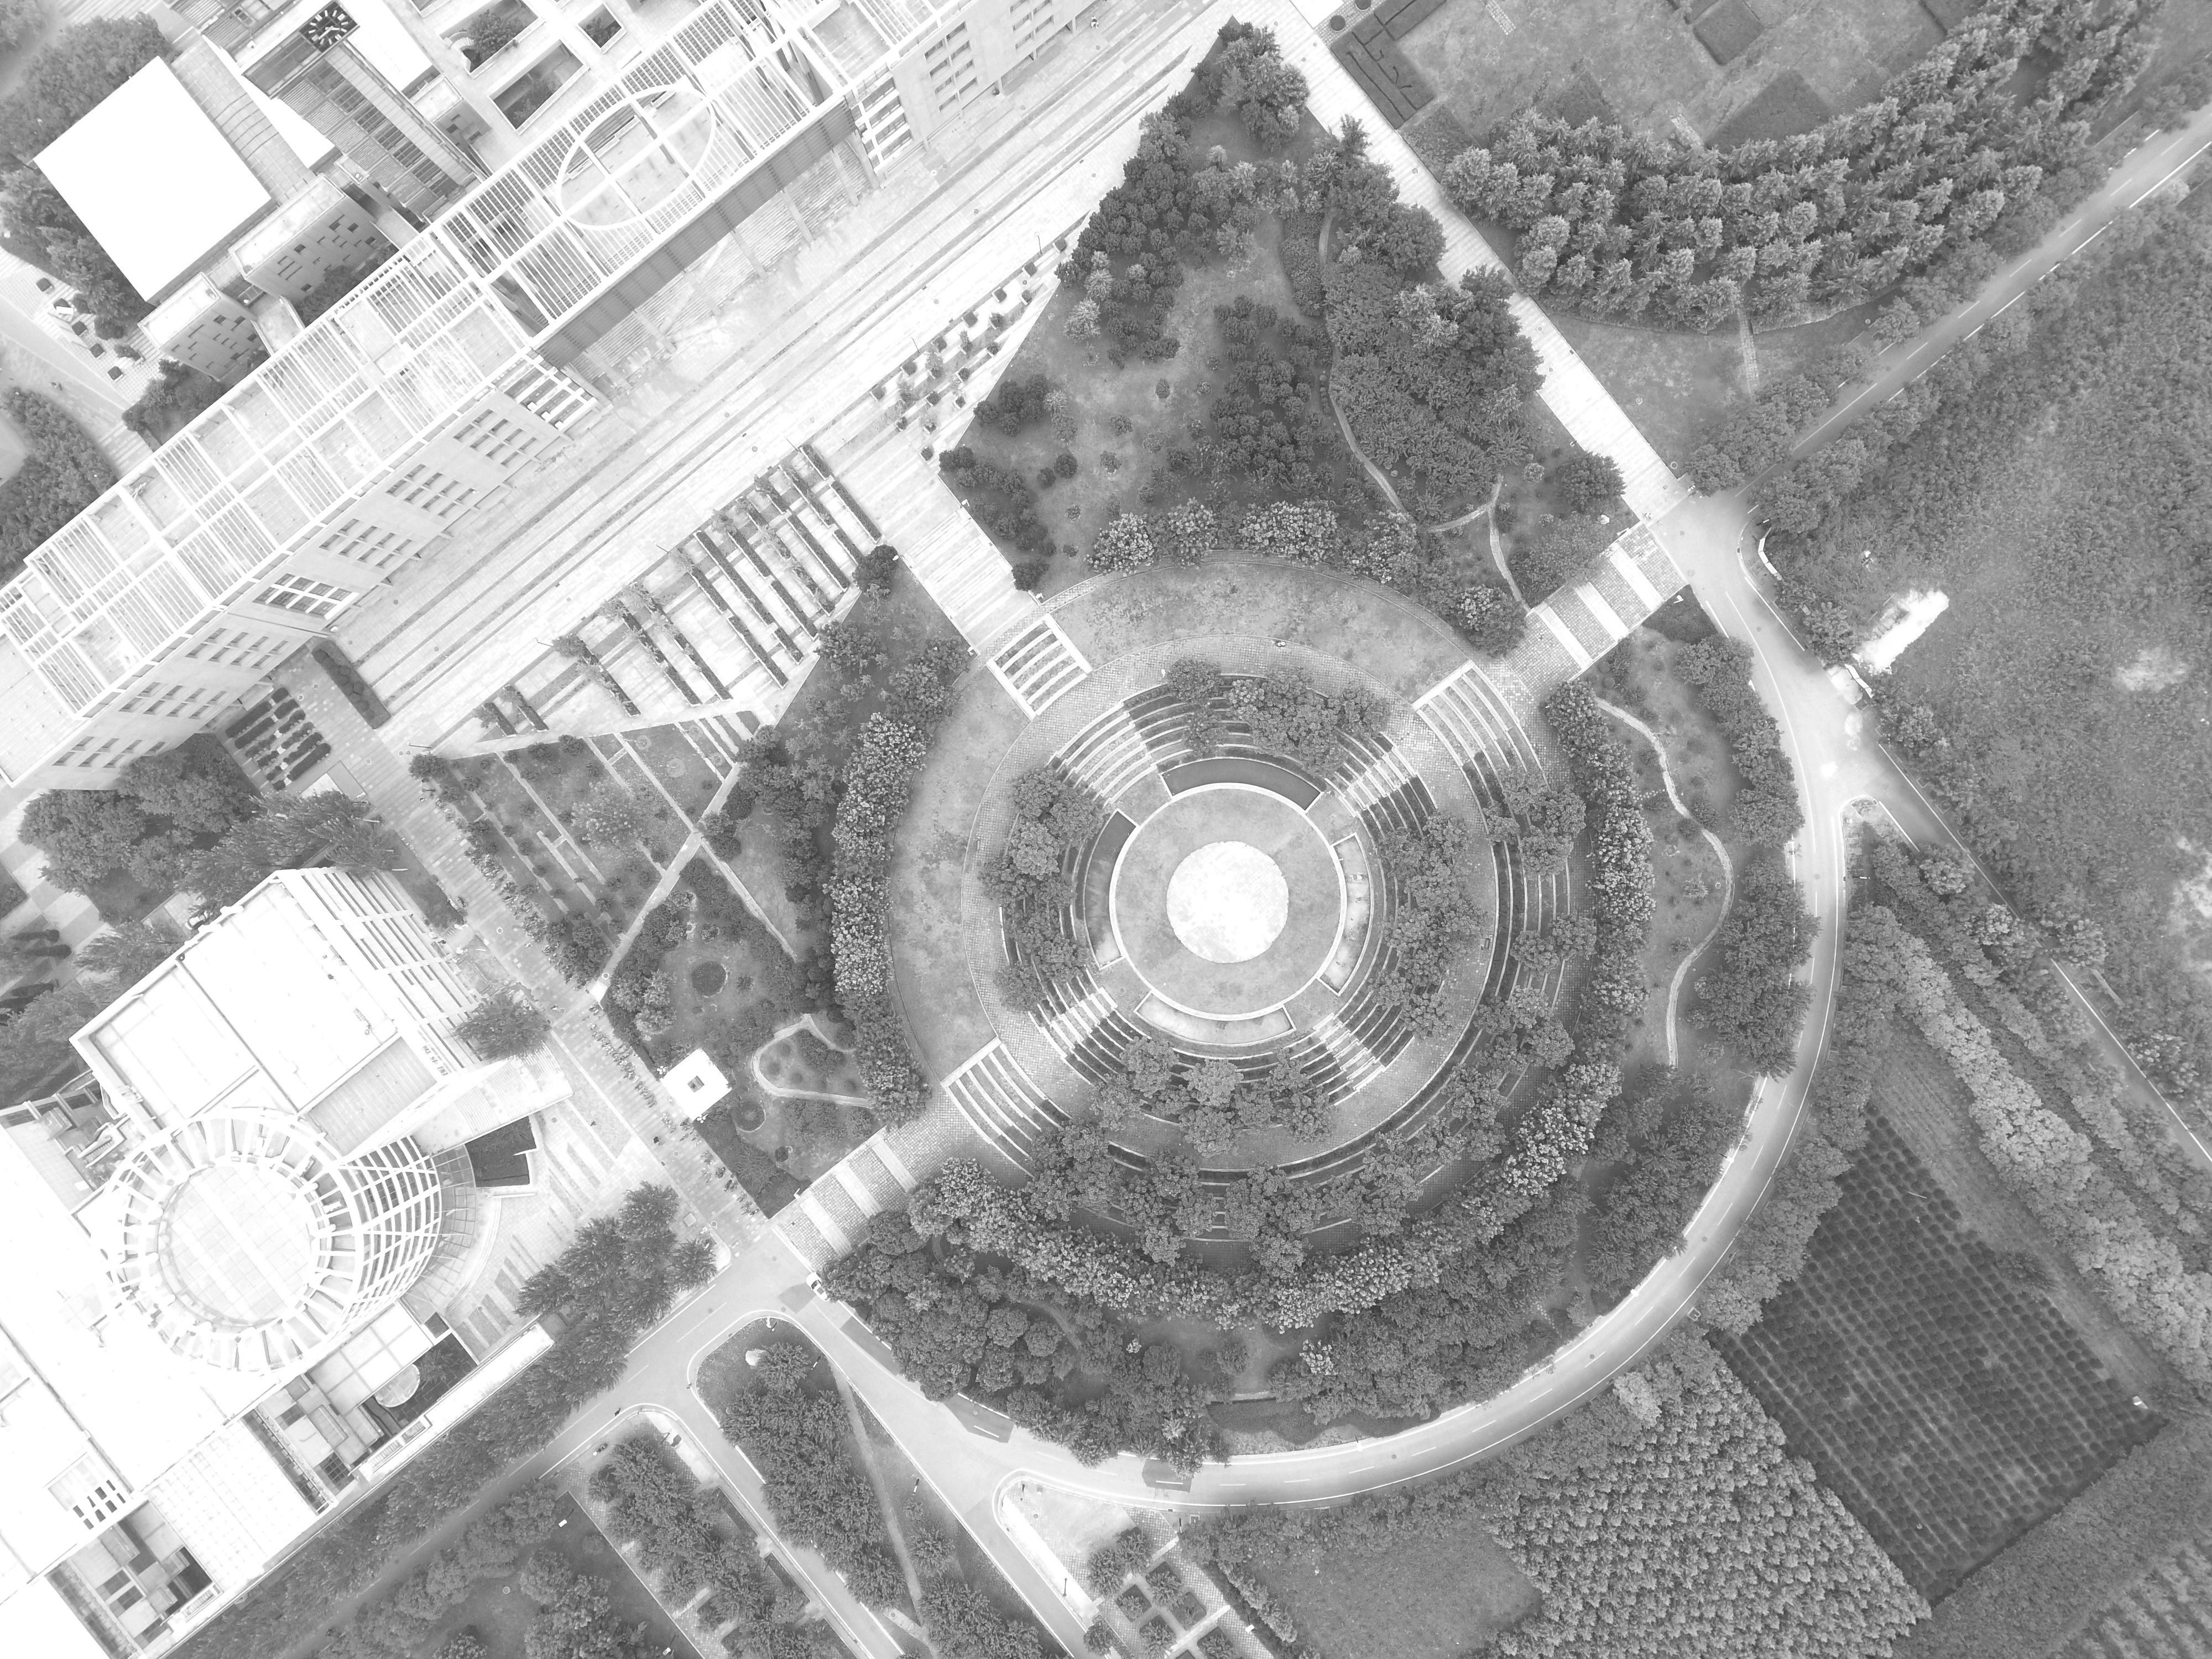
\includegraphics[width=\linewidth]{figure/DJI_0027_Energy.png}
		\caption{彩色图像的能量图像}
		\label{fig:dji0027energy}
	\end{minipage}
\end{figure}
\subsubsection{彩色图像的分解变换与合成}
对如图\ref{fig:dji0027original}所示的原图像进行红、绿、蓝通道进行分解,并且对红色分量增加高斯白噪声,对绿色分量进行$s=\log_{1.2}(1+0.2r)$的对数变换,对蓝色分量进行反转变换,可以得到如图\ref{fig:dji0027color_transform_fusion}所示的结果。
\begin{figure}[H]
	\centering
	\includegraphics[width=0.7\linewidth]{figure/DJI_0027_Transformed_Fusion.png}
	\caption{彩色图像的分解变换与合成结果}
	\label{fig:dji0027color_transform_fusion}
\end{figure}
\subsubsection{彩色图像两通道图像差异}
\begin{figure}[H]
	\centering
	\begin{minipage}{0.45\linewidth}
		\includegraphics[width=\linewidth]{figure/DJI_0027_Minus_Differ.png}
		\caption{采用$I_1=1-\min\left(\frac{\mu_1}{\mu_2},\frac{\mu_2}{\mu_1} \right) $计算差异图像的结果}
	\end{minipage}
	\begin{minipage}{0.45\linewidth}
		\includegraphics[width=\linewidth]{figure/DJI_0027_Log_Differ.png}
		\caption{采用$I_1=\left|\log X_1-\log X_2 \right| $计算差异图像的结果}
	\end{minipage}
\end{figure}
\subsubsection{差异图像的融合}
对以上两幅差异图像进行融合,可以得到如图\ref{fig:dji0027differ}所示的融合的差异图像。
\begin{figure}[H]
	\centering
	\includegraphics[width=0.7\linewidth]{figure/DJI_0027_Differ.png}
	\caption{差异图像的融合图像}
	\label{fig:dji0027differ}
\end{figure}
\subsubsection{标记兴趣区域}
假设我们对图片中的图书馆感兴趣,将图书馆设为兴趣区域,在对应的二值蒙版中将图书馆所在区域设置为“1”,其他部分设置为“0”。对图书馆所在的区域和其他区域进行不同的变换,再进行图像融合,即可突出图书馆在图片中的区域。
\begin{figure}[H]
	\centering
	\begin{minipage}{0.45\linewidth}
		\includegraphics[width=\linewidth]{figure/DJI_0027_Compressed_Mask.png}
		\caption{用于标记兴趣区域的二值蒙版}
	\end{minipage}
	\begin{minipage}{0.45\linewidth}
		\includegraphics[width=\linewidth]{figure/DJI_0027_Interest.png}
		\caption{突出兴趣区域的图像}
	\end{minipage}
\end{figure}
使用简单的灰度值平均或加权平均法融合的图像更符合人眼的直觉。简单的灰度值平均或加权平均法能够实现对不同区域和图像的明暗变化,能够更好地突出对不同区域亮度值的选择与区分。

使用简单的灰度值平均或加权平均法融合的图像可以控制要突出显示的目标轮廓、位置和纹理特征,适合小局部的目标辨别。差异图像的融合能够迅速地对全图的差异进行处理,适合大范围、零碎、没有明确边界特征和位置特征的目标的判断与识别,适合用于统计分析。
\end{document}